\subsection{Сбор и подготовка данных}\label{sect-3}

Для решения поставленной задачи первоначально был проведен опрос операторов БПЛА из ПСО "Лиза Алерт", и получены несколько примеров снимков. В результате, были выяснены следующие аспекты:

\begin{itemize}
    \item Условия съемки:
    \begin{itemize}
        \item Высота -- 40-50 метров над поверхностью земли;
        \item Съемка производиться вертикально (вид сверху);
        \item Во время съемки БПЛА зависает над сценой, чтобы сфокусироваться;
    \end{itemize}
    \item Позы, в которых чаще всего находят потерявшихся людей:
    \begin{itemize}
        \item Стоящий человек (идущий, бегущий);
        \item Сидячий человек (на корточках);
        \item Лежачий человек (на спине);
        \item Лежачий человек (на животе);
        \item Лежачий человек (на боку);
        \item Лежачий в позе эмбриона человек.
    \end{itemize}
\end{itemize}

При поиске доступных открытых решений удалось найти 2 набора данных (dataset-а): SDD (Stanford Drone Dataset) \cite{lib-sdd} и VisDrone DET dataset \cite{lib-visdrone}, но ни один из них не подходил для решения поставленной задачи (рис. \ref{sdd-visdrone-example}). В этих наборах данных несколько отличались условия съемки, а также, отсутствовали, как природная среда, так и интересующие нас позы. Однако, у них есть одно существенное преимущество -- они открыты и довольно распространены, а также, по схожести задачи они значительно ближе, чем какие-либо другие наборы данных. По этому, в описанных ниже исследованиях они использовались для предобучения моделей (а как следствие и сужения доменной области) и оценки качества моделей \cite{lib-transfer-learning}. Также, открытость этих данных и их известность позволила сравнивать качество полученных моделей с уже имеющимися.

\begin{figure}[H]
    \centering
    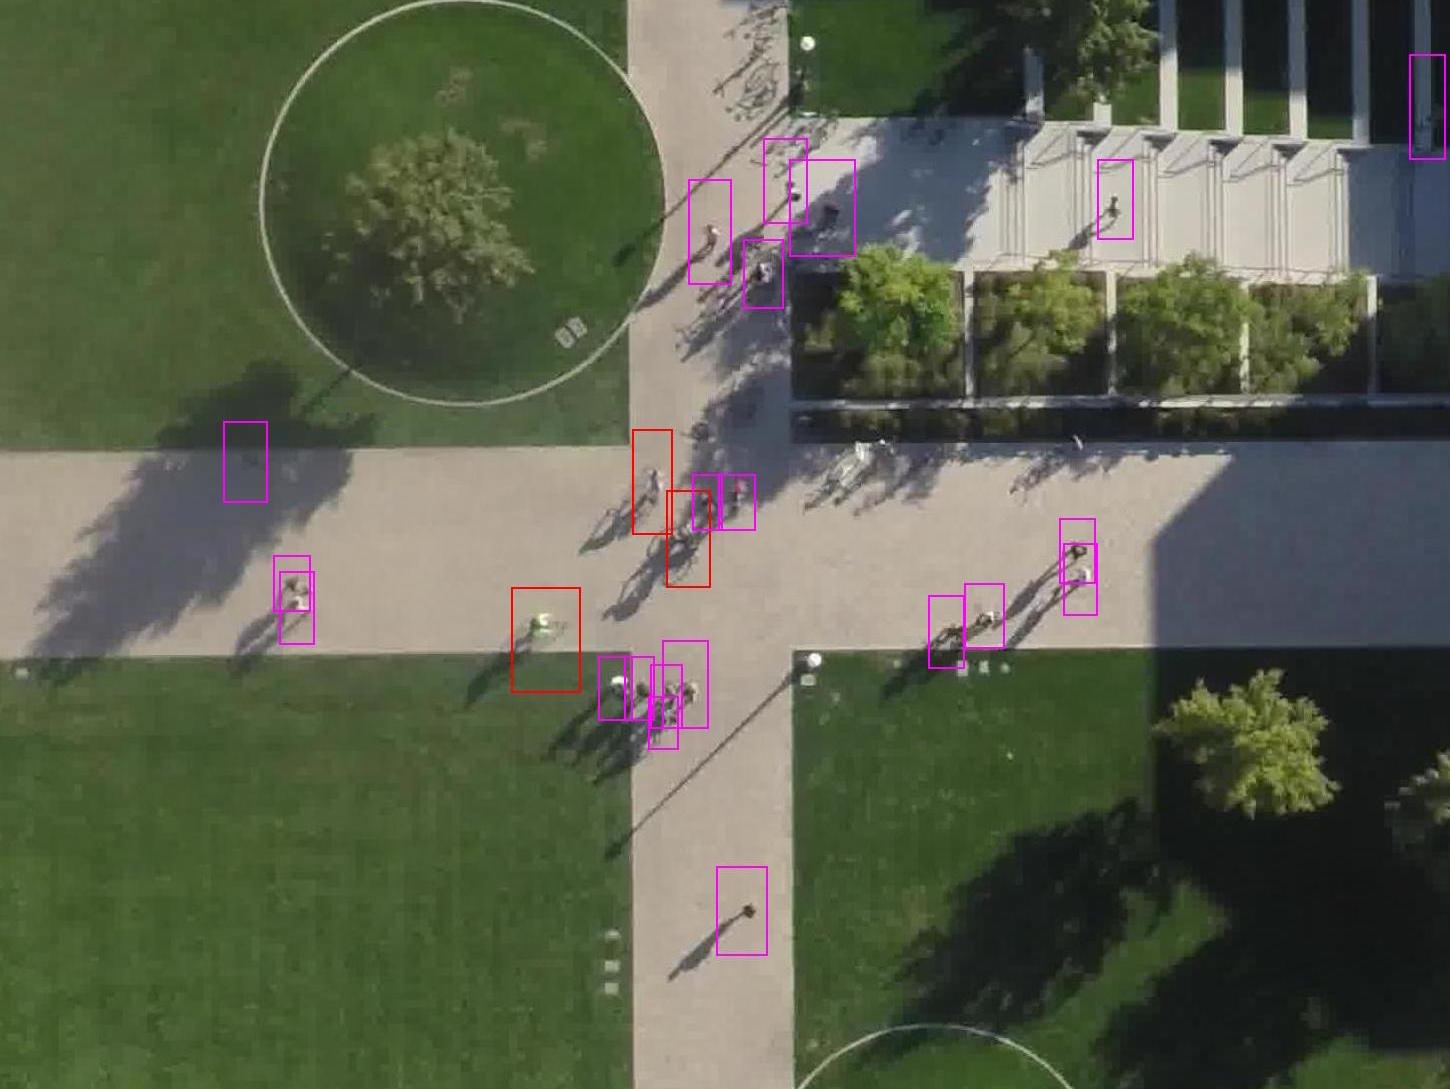
\includegraphics[width=0.42\linewidth]{3-sdd-example}
    \hfill
    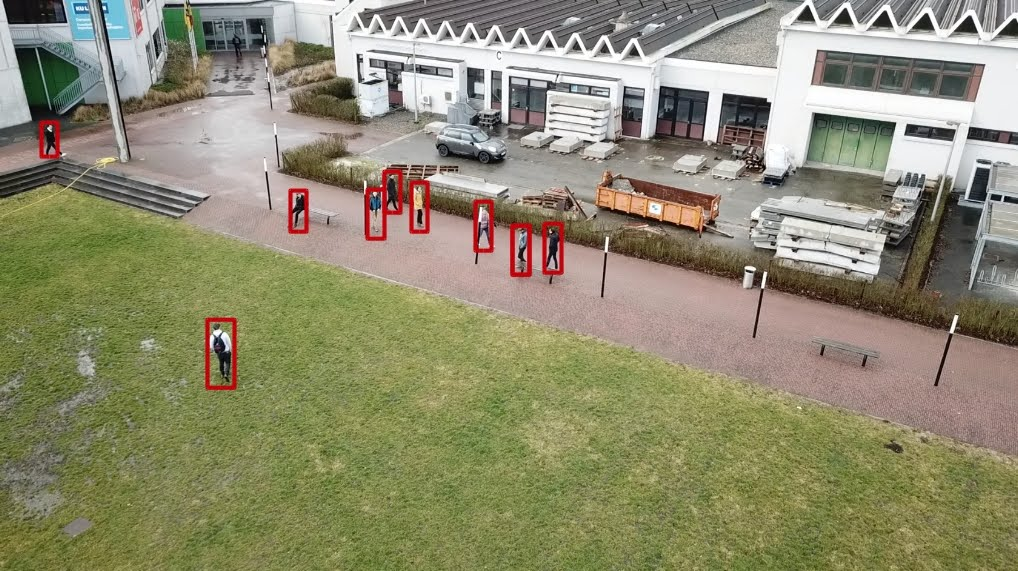
\includegraphics[width=0.56\linewidth]{3-visdrone-example}
    \caption{Примеры изображений SDD и VisDrone наборов данных} \label{sdd-visdrone-example}
\end{figure}


В силу специфичности решаемой задачи, пришлось самостоятельно формировать и организовывать сбор обучающей выборки с необходимыми нам фотографиями. Для решения этой задачи были привлечены добровольцы из различных ПСО, а также, разработаны методические материалы по сбору и разметке данных \cite{lib-lacmus-wiki-images}\cite{lib-lacmus-wiki-label}.

В результате был получен уникальный в своем роде набор данных, получивший в последствии название Lacmus Drone Dataset (LaDD) \cite{lib-ladd}. LaDD состоит из 1431 фотографии и имеет формат аннотирования Pascal VOC \cite{lib-pascal} с одним классом "Pedestrian" (пешеход). Dataset также является открытым и распространяется по лицензии GNU GPL v3. В его создании приняло участие множество ПСО из различных регионов России (Москва, Саратов, Ямал, Крым, Калининград и др). Таким образом, удалось достичь высокого разнообразия природных условий и, как следствие, обучающей выборки. Ниже приведен пример фотографии:

\addimghere{3-ladd-example}{1}{Московская область, осень 2019, бурелом, лежачий на боку человек}{ladd-example}